\documentclass{beamer}
\usetheme{Madrid}
\usecolortheme{default}
\usepackage{tikz} 
\usepackage{graphicx}
\graphicspath{ {./images} }

\usetikzlibrary{shapes,decorations,arrows,calc,arrows.meta,fit,positioning}
\tikzset{
    -Latex,auto,node distance =1 cm and 1 cm,semithick,
    state/.style ={ellipse, draw, minimum width = 0.7 cm},
    point/.style = {circle, draw, inner sep=0.04cm,fill,node contents={}},
    bidirected/.style={Latex-Latex,dashed},
    el/.style = {inner sep=2pt, align=left, sloped}
}

\title[Political Partisanship and EVs]
{Political Partisanship and Electric Vehicle Adoption in the US}

\author[Peter Shi] % (optional, for multiple authors)
{Peter Shi}

\date[March 2023] % (optional)
{March 2023}

\definecolor{uoftblue}{RGB}{6,41,88}
\setbeamercolor{titlelike}{bg=uoftblue}
\setbeamerfont{title}{series=\bfseries}

\begin{document}

\frame{\titlepage}

\section{Introduction and Motivation}

\begin{frame}
\frametitle{Introduction}
    \textbf{Background}. Electric Vehicles (EVs) are a key technology for the decarbonization of transportation. Recent literature has identified a wide array of factors affecting consumer adoption of EVs but the effect direction and magnitude of certain factors are poorly understood and require further investigation. \\~\\
    
    \textbf{Main Question}. How does political partisanship affect EV adoption? \\~\\
    
    \textbf{Hypothesis}. Negative relationships between county Republican vote share and EV adoption.

\end{frame}

\begin{frame}
\frametitle{Motivation}
    
\textbf{EV adoption has been steadily rising over the past few years, why bother with partisanship and EVs?}
\begin{enumerate}
\item Light vehicles account for a significant share of Greenhouse Gas emissions (15\% of total GHG in 2020 in the US)
    \begin{itemize}
        \item Internal Combustion Engines also emit other pollutants (Particulate Matter, NOX, Carbon Monoxide) that are linked to adverse public health outcomes
    \end{itemize}
\item Knowing the relationship between partisanship and EV adoption can help forecast adoption patterns more accurately
\item Despite political rhetoric, climate change is inherently bipartisan. Further investigation could inform better political decision-making 
    \begin{itemize}
        \item ex. Targeted subsidies, Tax rebates, or Infrastructure spending
    \end{itemize}
\end{enumerate}
\end{frame}

\section{Literature Review}

\begin{frame}
\frametitle{Meta-Analyses of EV adoption factors}
Coffman et al. (2016) and Anastasiadou and Gavanas (2022)

Factors:
\begin{itemize}
    \item Acquisition and Ownership Costs
    \item Vehicle Range
    \item Vehicle Charging Time
    \item Fuel/Electricity Prices
    \item \textbf{Consumer Characteristics}
    \item Distances Travelled 
    \item Infrastructure 
    \item Policy Mechanisms
\end{itemize}
\end{frame}

\begin{frame}
\frametitle{Literature Review}

\begin{itemize}
    \item \structure{Hayashida et al. (2021):} governors and state legislatures were not significant for state EV subsidies but significant for household charger subsidies. Panel OLS model with state and year fixed effects.
    \item \structure{Sintov et al. (2020):} democrats were more likely to adopt EVs compared to republicans. Biased survey with a small sample (N = 545).
    \item \structure{Adua and Clark (2020):} significant relationship between governorship and congressional delegation on state-level electric utility efficiency. 4SLS OLS model with clustered errors. But EV adoption occurs in a much more decentralized manner compared to electrical infrastructure.
\end{itemize}
\end{frame}

\begin{frame}
\frametitle{Literature Review (Economics)}

\begin{itemize}
    \item \structure{Beresteanu and Li (2011):} Strong positive effect of fuel prices on Hybrid EV sales.
    \item \structure{Gallagher and Muehlegger (2011):} Significant effect of Tax Incentives and Fuel prices on EV purchases, insignificant effect of HOV lane access.
    \item \structure{Bushnell et al. (2022):} Gasoline prices have a larger effect on demand for EVs than electricity prices (4x-6x the effect size).
    \item \structure{Archsmith et al. (2021):} Projects future scenarios of EV adoption. Does mention partisan bias and preference for sedans versus trucks but effect sizes were not estimated.
\end{itemize}
\end{frame}

\begin{frame}
\frametitle{Methodology}
\begin{itemize}
    \item \structure{Units:} US Counties 
    \item \structure{Dependent Variable:} EV Share of Total Vehicles Registered in County
    \item \structure{Independent Variable:} Republican vote share in counties in the 2016 federal election, $\Delta$ in 2020 federal election
    \item \structure{Control Variables:} State Partisanship (Governor, Legislature), County Demographics (Income, Education, Population, Poverty), Charging Infrastructure, fuel price
\end{itemize}
\end{frame}

\begin{frame}
\frametitle{Methodology}

\textbf{Proposed Model:} Panel OLS with Controls and Fixed effects

\vspace{5mm}

\centering
$
{EV Proportion_{t,c}} = \alpha + \beta_{1} fed pol_{2016,c} + \beta_{2} \Delta fed pol_{2020,c} +\theta STATE POL_{t,s} +\delta  DEMOG_{c} + \kappa  infra_{t,c} + \omega fuelprice_{t} + \gamma_{t} + \tau_{s} +\epsilon
$

\vspace{5mm}

\raggedright

\textbf{Problem:} Endogeneity between voting patterns and EV adoption

\end{frame}

\begin{frame}
\frametitle{Methodology}
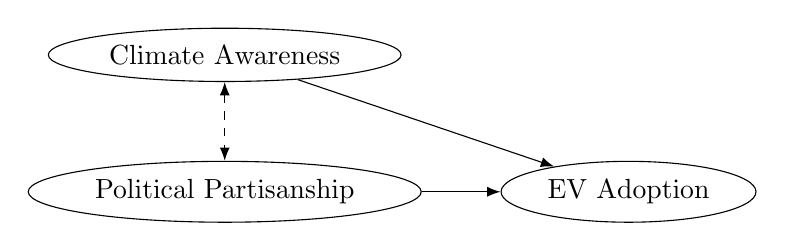
\begin{tikzpicture}

    \node[state] (pol) at (0,0) {Political Partisanship};

    % y node set relative to x.
    % Locations can be:
    % right,left,above,below,
    % above left,below right, etc
    \node[state] (EV) [right = of pol] {EV Adoption};

    \node[state] (clim) [above = of pol] {Climate Awareness};

    % Directed edge
    \path (pol) edge (EV);

    % Bidirected edge
    \path[bidirected] (clim) edge (pol);
    \path (clim) edge (EV);


\end{tikzpicture}
\end{frame}

\begin{frame}
\frametitle{Methodology}
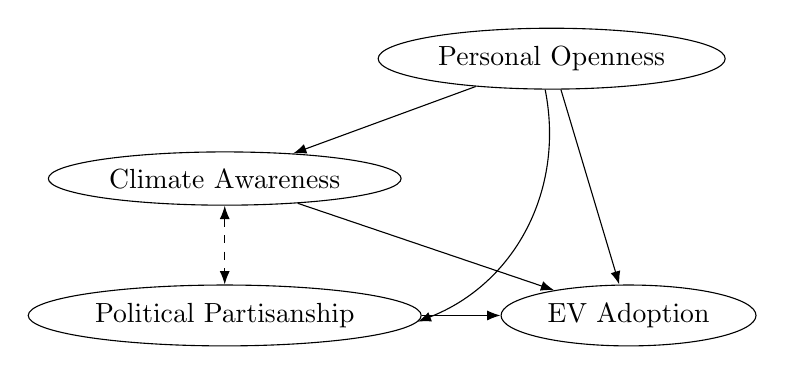
\begin{tikzpicture}

    \node[state] (pol) at (0,0) {Political Partisanship};

    % y node set relative to x.
    % Locations can be:
    % right,left,above,below,
    % above left,below right, etc
    \node[state] (EV) [right = of pol] {EV Adoption};

    \node[state] (clim) [above = of pol] {Climate Awareness};

    \node[state] (open) [above right = of clim] {Personal Openness};

    % Directed edge
    \path (pol) edge (EV);

    % Bidirected edge
    \path[bidirected] (clim) edge (pol);
    \path (open) edge[bend left=40](pol);
    \path (open) edge (clim);
    \path (clim) edge (EV);
    \path (open) edge (EV);


\end{tikzpicture}
\end{frame}

\begin{frame}
\frametitle{Methodology}
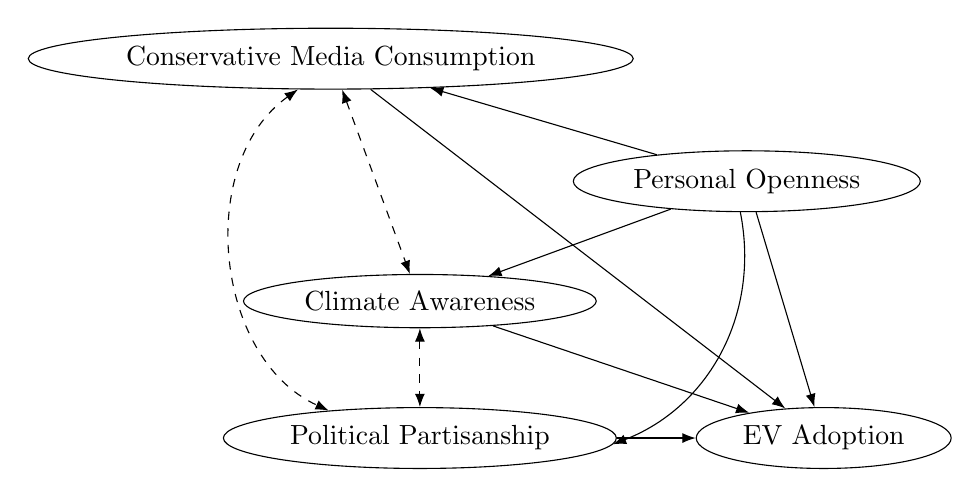
\begin{tikzpicture}

    \node[state] (pol) at (0,0) {Political Partisanship};

    % y node set relative to x.
    % Locations can be:
    % right,left,above,below,
    % above left,below right, etc
    \node[state] (EV) [right = of pol] {EV Adoption};

    \node[state] (clim) [above = of pol] {Climate Awareness};

    \node[state] (open) [above right = of clim] {Personal Openness};

    \node[state] (conmedia) [above left = of open] {Conservative Media Consumption};

    % Directed edge
    \path (pol) edge (EV);

    % Bidirected edge
    \path[bidirected] (clim) edge (pol);
    
    \path (open) edge[bend left = 40](pol);
    \path (open) edge (clim);
    \path (open) edge (conmedia);
    
    \path[bidirected] (conmedia) edge (clim);
    \path[bidirected] (conmedia) edge[bend right = 60] (pol);
    
    \path (conmedia) edge (EV);
    \path (clim) edge (EV);
    \path (open) edge (EV);


\end{tikzpicture}
\end{frame}

\begin{frame}
\frametitle{Methodology}

\textbf{A Brief Aside:} 

\vspace{5mm}

I don't think how a particular county votes \textbf{in isolation} has any causal relationship with EV adoption. It's just a proxy metric for American Republican ideology which encompasses all the aforementioned confounders. 

\vspace{5mm}

\begin{alertblock}{My Point} 
A proxy metric needs Endogeneity to be a good proxy. But at what point does Endogeneity become a problem?
\end{alertblock}

\end{frame}

\begin{frame}
\frametitle{Methodology}

\textbf{Possible Remedies:} 

\vspace{5mm}

\begin{itemize}
    \item Find an Instrument (Difficult) 
    \\
    \vspace{5mm}
    AND/OR
    \vspace{5mm}
    \item Specify a different question/regression with the same dataset
\end{itemize}

\vspace{5mm}

Open to suggestions

\end{frame}

\begin{frame}
\frametitle{Data}

\begin{itemize}
    \item \structure{County Partisanship:} Election returns in the 2016 and 2020 federal elections. Published by the MIT Election Data Lab
    \item \structure{State Partisanship:} Governor and Legislature partisanship. Scraped from the National Governors Association and Ballotpedia respectively
    \item \structure{EV Population:} Monthly county-level vehicle population grouped by vehicle class (passenger vs truck) and drivetrain (electric, hybrid, non-electric). Published by State of Washington Department of Licensing
    
\end{itemize}

\end{frame}

\begin{frame}
\frametitle{Data}

\begin{itemize}
    \item \structure{Demographics:} County-level Population, Education, Unemployment, and Poverty from census data. Published by the Economic Research Service of the US Department of Agriculture
    \item \structure{Fuel Price:} Monthly US mean gasoline price (\$/gallon). Published by the Federal Highway Administration of the US Department of Transportation
    \item \structure{Charging Station:} County-level station count. Published by the Alternative Fuels Data Center of the US Department of Energy

    \vspace{5mm}

    Merged and Processed with Python (Pandas)

    \vspace{5mm}

    Spatial Merging (ZIP-code to County) done with U.S. Department of Housing and Urban Development's Crosswalk Files 
    
\end{itemize}

\end{frame}

\begin{frame}
\frametitle{Summary Statistics}

\begin{figure}[!htb]
  \includegraphics[width=\textwidth]{countypop}
  \caption{Number of Counties counted}
\end{figure}
\end{frame}

\begin{frame}
\frametitle{Summary Statistics}

\begin{figure}[!htb]
  \includegraphics[width=\textwidth]{popcounted}
  \caption{Population Counted}
\end{figure}

\end{frame}

\begin{frame}
\frametitle{Summary Statistics}

\begin{figure}[!htb]
  \includegraphics[width=\textwidth]{evpop}
  \caption{Average EV population as a \% of total vehicle population}
\end{figure}

\end{frame}

\begin{frame}
\frametitle{Summary Statistics}

\begin{figure}[!htb]
  \includegraphics[width=\textwidth]{elechist}
  \caption{Histogram of County Republican Vote Share in 2016 US Federal Election}
\end{figure}

\end{frame}

\begin{frame}
\frametitle{Summary Statistics}

\begin{figure}[!htb]
  \includegraphics[width=\textwidth]{incomehist}
  \caption{Histogram of County Median 2020 income}
\end{figure}

\end{frame}

\begin{frame}
\frametitle{Preliminary OLS Results}

All regressions run with linearmodels.PanelOLS

\vspace{5mm}

\textbf{Base Case Regression:}

\vspace{5mm}

\begin{center}

\begin{tabular}{lcccccc}
                       & \textbf{Parameter} & \textbf{Std. Err.} & \textbf{T-stat} & \textbf{P-value} \\
\midrule

\textbf{const}         &       4184.5       &       369.88       &      11.313     &      0.0000      \\  
\textbf{percent\_rep}  &      -4193.5       &       399.51       &     -10.497     &      0.0000      \\
\textbf{percentchange} &      -1932.5       &       192.25       &     -10.052     &      0.0000      \\
\bottomrule
\end{tabular}
%\caption{PanelOLS Estimation Summary}
\end{center}

F-test for Poolability: 110.71 \newline
P-value: 0.0000 \newline
Distribution: F(51,12635) 
\newline
\newline
Included effects: State, Year

\end{frame}

\begin{frame}
\frametitle{Preliminary OLS Results}

\textbf{Regression with demographic controls:}

\vspace{5mm}

\begin{center}

\begin{tabular}{lcccccc}
                                                                      & \textbf{Parameter} & \textbf{Std. Err.} & \textbf{T-stat} & \textbf{P-value} \\
\midrule
\textbf{const}                                                        &       2109.4       &       228.19       &      9.2443     &      0.0000       \\
\textbf{percent\_rep}                                                 &      -3387.7       &       221.09       &     -15.322     &      0.0000      \\
\textbf{percentchange}                                                &      -2211.2       &       234.93       &     -9.4120     &      0.0000      \\
\textbf{Median\_HH\_Income}                                           &       0.0349       &       0.0033       &      10.604     &      0.0000     \\
\textbf{Percent w/ a bachelor}                                        &      -19.207       &       1.8533       &     -10.363     &      0.0000     \\
\textbf{Population 2021}                                              &       0.0004       &     4.524e-05      &      8.6449     &      0.0000      \\
\textbf{PCTPOVALL\_2020}                                              &      -14.712       &       5.7036       &     -2.5794     &      0.0099      \\
\bottomrule
\end{tabular}
%\caption{PanelOLS Estimation Summary}
\end{center}

F-test for Poolability: 117.54 \newline
P-value: 0.0000 \newline
Distribution: F(51,12631) \newline
\newline
Included effects: State, Year
\end{frame}

\begin{frame}
\frametitle{Preliminary OLS Results}

\begin{center}

\begin{tabular}{lcccccc}
                                                                      & \textbf{Parameter} & \textbf{Std. Err.} & \textbf{T-stat} & \textbf{P-value} \\
\midrule
\textbf{const}                                                        &       4169.7       &       494.55       &      8.4311     &      0.0000     \\
\textbf{percent\_rep}                                                 &      -3492.3       &       237.54       &     -14.702     &      0.0000      \\
\textbf{percentchange}                                                &      -2409.5       &       268.92       &     -8.9599     &      0.0000     \\
\textbf{\%\_rep\_house}                                               &      -3949.4       &       630.23       &     -6.2666     &      0.0000      \\
\textbf{rep\_maj\_house}                                              &       245.98       &       88.293       &      2.7859     &      0.0053      \\
\textbf{rep\_supmaj\_house}                                           &      -107.74       &       91.382       &     -1.1790     &      0.2384      \\
\textbf{\%\_rep\_sen}                                                 &      -229.63       &       575.62       &     -0.3989     &      0.6900      \\
\textbf{rep\_maj\_sen}                                                &       213.41       &       80.822       &      2.6405     &      0.0083      \\
\textbf{rep\_supmaj\_sen}                                             &       227.36       &       67.303       &      3.3782     &      0.0007      \\
\textbf{rep\_gov}                                                     &       78.223       &       48.151       &      1.6245     &      0.1043      \\
\textbf{Median\_HH\_Income}                                           &       0.0346       &       0.0032       &      10.721     &      0.0000      \\
\textbf{Percent w/ a bachelor}                                        &      -22.111       &       1.8248       &     -12.117     &      0.0000      \\
\textbf{Population 2021}                                              &       0.0002       &      3.29e-05      &      7.1229     &      0.0000      \\
\textbf{PCTPOVALL\_2020}                                              &      -14.251       &       5.7814       &     -2.4650     &      0.0137      \\
\textbf{n\_charging\_stations}                                        &       1.5910       &       0.5004       &      3.1796     &      0.0015      \\
\textbf{Gas Prices (\$/Gallon)}                                       &       13.387       &       99.325       &      0.1348     &      0.8928      \\
\bottomrule
\end{tabular}

%\caption{PanelOLS Estimation Summary}
\end{center}
\end{frame}

\begin{frame}
\frametitle{Preliminary Interpretations}
\begin{itemize}
    \item Economically and statistically significant negative effect size of county partisanship and $\Delta$ partisanship on EV registrations
    \item Negative effect for county education (Surprising)
    \item Positive effect for Republican state house majority, and Republican state senate majority and supermajority (Surprising)
    \item Insignificant effect size for Gasoline price, but the data I have isn't very good
\end{itemize}


\end{frame}

\begin{frame}
\frametitle{Next Steps}

\begin{itemize}
    \item Collect + process more data (Vehicle Miles Travelled, Subsidies and other incentives, Better Gas Price Data)
    \item Consider finding an instrument 
    \item Consider different questions with the same dataset
    \item Consider same regression but with different fixed effects (Month, County) - worried there is not enough data within each group 
    \item Open to suggestions
\end{itemize}

\end{frame}

\begin{frame}
\frametitle{Next Steps}
\centering
Questions?
\end{frame}

\end{document}